\documentclass[tikz,crop,convert={density=300,outext=.png},border=0.0cm,width=18cm,height=3cm]{standalone}
\usepackage{pgfplots}
\usepackage{amsmath}
\usepackage{physics}

\definecolor{symmetry_colour}{RGB}{102,37,6}
\definecolor{one}{RGB}{0,68,27}
\definecolor{two}{RGB}{35,139,69}
\definecolor{three}{RGB}{153,216,201}
\definecolor{mixed_1}{RGB}{2,56,88}
\definecolor{mixed_2}{RGB}{54,144,192}
\definecolor{mixed_3}{RGB}{208,209,230}
\definecolor{pow_1}{RGB}{0,68,27}
%\definecolor{pow_1}{RGB}{103,0,31}
\definecolor{pow_2}{RGB}{206,18,86}
\definecolor{pow_3}{RGB}{223,101,176}
\pgfplotsset{compat=newest,
    %width=6cm,
    %height=3cm,
    scale only axis=true,
    max space between ticks=25pt,
    try min ticks=5,
    every axis/.style={
        axis y line=middle,
        axis x line=middle,
        axis line style={thick,->,>=latex, shorten >=-.3cm}
    },
      every axis plot/.append style={thick},
    tick style={black, thick},
}
\tikzset{
    semithick/.style={line width=0.8pt},
  }
\usetikzlibrary{shapes.geometric, arrows}  
\usepgfplotslibrary{groupplots}
\usepgfplotslibrary{dateplot}
\usetikzlibrary{positioning}
%\pgfplotsset{compat=1.17}

\tikzstyle{mod_sel} = [rectangle, rounded corners, minimum width=2cm, minimum height=1cm,text centered, draw=black, fill=one]
\tikzstyle{PLM} = [rectangle, rounded corners, minimum width=1cm, minimum height=1cm,text centered, draw=black, fill=pow_1]
\tikzstyle{IM-III} = [rectangle, rounded corners, minimum width=1cm, minimum height=1cm,text centered, draw=black, fill=mixed_1]
\tikzstyle{symmetry} = [rectangle, rounded corners, minimum width=1cm, minimum height=1cm,text centered, draw=black, fill=symmetry_colour]
\tikzstyle{arrow} = [ultra thick,->,>=latex]


\begin{document}
\begin{tikzpicture}

%==============================================================================================================================================
  \node[inner sep=0pt] (stab_r) at (-4.00,3.50)
  {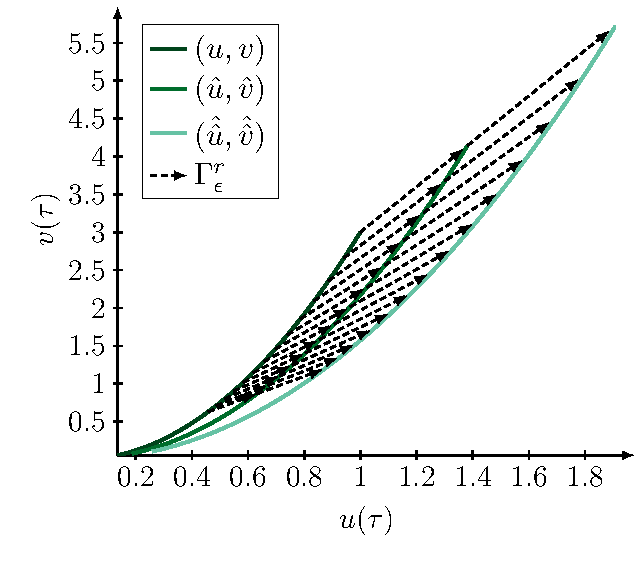
\includegraphics[width=8cm,page=1]{{./individual_figures_linear_symmetries}}};
    \node[inner sep=0pt] (stab_theta) at (4.00,3.50)
    {\includegraphics[width=8cm,page=2]{{./individual_figures_linear_symmetries}}};
      \node[inner sep=0pt] (saddle_r) at (-4.00,-3.50)
  {\includegraphics[width=8cm,page=3]{{./individual_figures_linear_symmetries}}};
    \node[inner sep=0pt] (saddle_theta) at (4.00,-3.50)
 {\includegraphics[width=8cm,page=4]{{./individual_figures_linear_symmetries}}};

  \node[color=white,align=center] (PLM) at (-9.15,4.25) [PLM] {Stable node\\$A=\begin{pmatrix}-1 & 0\\ 0 & -2\end{pmatrix}$};
  \node[color=white,align=center] (IM-III) at (-9.15,-2.75) [IM-III] {Saddle point\\$A=\begin{pmatrix}1 & 0\\ 0 & -2\end{pmatrix}$};
    \node[color=white,align=center] (PLM) at (-3.15,8.15) [symmetry] {Radial symmetry $\Gamma_{\epsilon}^{r}$};
  \node[color=white,align=center] (IM-III) at (4.75,8.15) [symmetry] {Angular symmetry $\Gamma_{\epsilon}^{\theta}$};

\end{tikzpicture}

\end{document}
